%FIR Filter Module

\subsubsection{Overview}
\label{FIR Filter}
\index{FIR Filter}\index{utilities, FIR Filter}\index{filter, FIR Filter}

\begin{figure}[h]
\begin{center}
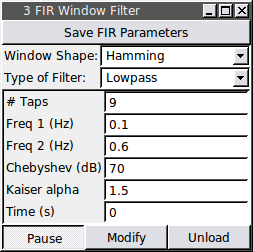
\includegraphics[width=2in]{FIRwindow.png} 
\caption[firfilter]{The wave maker module allows the output of a pre-recorded signal from an ASCII file.} 
\end{center}
\label{firfilter}
\end{figure}

The Finite Impulse Response Filter module creates an in-line FIR filter that can be applied to any signal in RTXI. Given the desired number of filter taps (filter order + 1), it computes the impulse response for a lowpass, highpass, bandpass, or bandstop filter using the window method. For a lowpass or highpass filter, the module uses the first frequency as the cut-off frequency. For a bandpass or bandstop filter, both input frequencies are used to define the frequency band. The module initially computes an ideal FIR filter to which you can apply a Triangular (or Bartlett), Hamming, Hann, Kaiser, or Dolph-Chebyshev window. The Hann window is not to be confused with the Hanning window (see MATLAB’s hann() vs. hanning() functions). To apply no window to the filter, choose the Rectangular filter. The Kaiser and Chebyshev windows each take a parameter that determines the attenuation of the sidelobes in the filter. The algorithms only accept an odd number of filter taps. If an even number is entered, the module will automatically add 1 to the number of filter taps.

\subsubsection{Input Channels}
\begin{description}
\item [Input]Signal to be filtered
\end{description}

\subsubsection{Output Channels}
\begin{description}
\item [Output]Filtered input signal
\end{description}

\subsubsection{Parameters}
\begin{description}
\item [Window Shape]  
  \begin{itemize}
  \item Rectangular
  \item Triangular (Bartlett)
  \item Hamming
  \item Hann
  \item Chebyshev
  \item Kaiser
  \end{itemize}
\item [Type of Filter]
  \begin{itemize}
  \item Highpass
  \item Lowpass
  \item Bandpass
  \item Bandstop
  \end{itemize}
\item [\# Taps]
\item [Freq 1 (Hz)]
\item [Chebyshev (dB)]
\item [Kaiser alpha]
\end{description}

\subsubsection{States}
\begin{description}
\item [Time (s)] Time elapsed, in seconds, since filter was started
\end{description}